% Title:  pc1.graphe
%
% Doc: /users/enstb1/thesards/brucker/Tex/pc1.graphe.tex
% Original Author:     BRUCKER Francois
% Created:             Tue Nov 30 1999
%

\documentclass
[12pt]
{article}
\usepackage[utf8]{inputenc}

\usepackage{amssymb}
\usepackage[ruled, vlined, french]{algorithm2e}
\usepackage[pdftex]{graphicx}

\usepackage{fullpage} \usepackage{setspace}

\begin{document}

\begin{center}
  \begin{tabular}{c}
  \hline\\%\vspace{0.1cm}
  {\textsc{mpcI}}\vspace{0.1cm}
  \\
%  
    {\bf {\Large Programmation 2}}\\\vspace{0.2cm}
    {\bf  { Examen Final}}\\
    {\footnotesize Mercredi 4 mars 2020}\\
    \hline
  \end{tabular}
\end{center}
\vspace{0.6cm}
%
%
{\em On rappelle qu'aucun document ni équipement électronique n'est autorisé. L'usage du thermomètre à mercure est néanmoins toléré. La clarté \& la concision des réponses sera appréciée. Les algorithmes doivent {\bf tous} être prouvés {\bf et} donnés avec leur complexité.}\\

{\em L'examen est composé de 5 exercices indépendants valant chacun 4 pts.}\\

\begin{description}
\item[Exercice 1~:] On souhaite recherche si un entier \texttt{e} est dans une liste triée d'entiers \texttt{L}. Ecrivez un algorithme utilisant la méthode dichotomique pour résoudre ce problème. \\


%
\item[Exercice 2~:] Un {\it col} dans une matrice est un élément qui est le plus petit de sa colonne \& le plus grand de sa ligne.
\begin{enumerate}
\item Est-ce que toute matrice admet un col~?
\item Est-ce que certaines matrices admettent un col~?
\item Ecrivez un algorithme qui détermine si une matrice admet un col \& qui, dans le cas positif, donne ses coordonnées (ligne \& colonne).\\
\end{enumerate}

%
%

\item[Exercice 3~:] Un morceau (musique, vidéo, \dots) est représenté par un objet d’une classe \texttt{Morceau} précisant son titre et sa durée. Ces deux informations seront transmises au moment de la construction de l’objet.
\begin{enumerate}
    \item  Donnez le code python de la classe \texttt{Morceau}.
    \item Ecrivez en python un programme principal (c’est à dire que l’on suppose la classe Morceau déjà écrite) qui crée un Morceau dont le titre est {\it Stupeflip, vite !} d’une durée de 3 minutes 39.
    \item Une \texttt{Playlist} est composée d’une liste de Morceaux de musique ou de vidéos. On créera une
Playlist en précisant une liste de Morceaux. Donnez le code python de cette classe.
    \item Ajoutez une méthode nommée \texttt{morceau} à la classe \texttt{Playlist} qui rend le morceau dont le nom est passé en paramètre (ou \texttt{None} si le morceau n'existe pas).
\end{enumerate}

\item[Exercice 4~:] On considère $n.p$ entiers positifs $a_{ij}$ ($0\leq i< n, 0\leq
j< p$), écrits sur un cylindre ayant $n$ lignes \& $p$ colonnes,
comme illustré ci-dessous.%figure \ref{CYLINDRE}.
%
\begin{figure}[h!]
\begin{center}
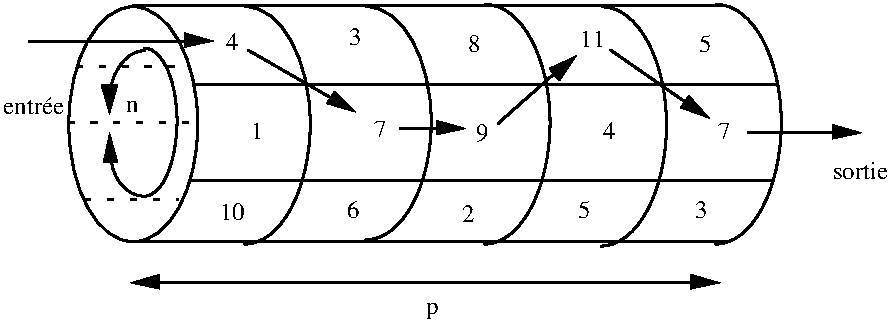
\includegraphics[scale=0.5]{Cyl1}
%\caption{\label{CYLINDRE}Un cylindre} 
\end{center}
\end{figure}
Un chemin est tracé de l'entrée du cylindre jusqu'à la sortie, avec la
restriction que, d'une case, on ne peut aller qu'aux trois positions
de la colonne suivante adjacentes à la position courante. Le coût d'un
tel chemin est la somme des entiers écrits dans les cases traversées
(par exemple, le chemin tracé sur le dessin a un coût égal à 38).

\begin{enumerate}
\item {Combien} de chemins distincts a-t-on de l'entrée à la
sortie, les cases de départ \& d'arrivée n'étant pas imposées ?



\item {Donner} un algorithme récursif qui détermine un tel chemin, de
coût minimum On justifiera le fait
que l'algorithme calcule bien ce qu'il faut, \& on donnera   sa complexité.\\
{\it Indication}~: Un chemin arrivant à la case $a_{i,j}$ passe forcément par une des cases $a_{i,j-1}$, $a_{i-1,j-1}$ ou $a_{i+1,j-1}$ (les opérations sur $i$ sont faites modulo $n$).

\item Transformer cet algorithme en un algorithme itératif de complexité $O(np)$.

\item {L'appliquer} à l'exemple de la figure % \ref{CYLINDRE} 
où l'on suppose que l'on voit tout le cylindre
($n=3$, $p=5$)~;
en déduire un chemin de coût minimum.
\end{enumerate}

\item[Exercice 5~:] La suite de Fibonacci est définie par $F_0 = 0$, $F_1= 1 $, \& $F_{i+2} = F_{i+1} + F_i$ pour $i \in N$ 
\begin{enumerate}
\item Donner un algorithme récursif \& un algorithme itératif pour calculer $F_i$. 

\item Comparer ces deux algorithmes.
\end{enumerate}

\end{description}


\end{document}


%%% Local Variables: 
%%% mode: latex
%%% TeX-master: t
%%% End: 
